\documentclass[aspectratio=169]{beamer}\usepackage[utf8]{inputenc}
\usepackage[english]{babel}
\usepackage{color}
\usepackage{amsmath,mathtools}
\usepackage{mathptmx}
\usepackage[11pt]{moresize}
\setbeamertemplate{navigation symbols}{}
\setbeamersize{text margin left=5mm,text margin right=5mm}
\usepackage{wrapfig}
\usepackage{bbm}
\usepackage{xcolor}
\usepackage{tabularx}
\usepackage{bm}
\usepackage{lmodern}
\usepackage{algorithm2e}


\newcommand{\R}{\mathbb{R}}
\newcommand{\E}{\mathbb{E}}
\newcommand{\N}{\mathbb{N}}
\newcommand{\Z}{\mathbb{Z}}
\newcommand{\V}{\mathbb{V}}
\newcommand{\Q}{\mathbb{Q}}
\newcommand{\K}{\mathbb{K}}
\newcommand{\C}{\mathbb{C}}
\newcommand{\T}{\mathbb{T}}
\newcommand{\I}{\mathbb{I}}

\setbeamertemplate{caption}[numbered]

\addtobeamertemplate{navigation symbols}{}{%
    \usebeamerfont{footline}%
    \usebeamercolor[fg]{footline}%
    \hspace{1em}%
    \insertframenumber/\inserttotalframenumber
}

\setbeamercolor{footline}{fg=blue}
\setbeamerfont{footline}{series=\bfseries}



\title{Uncertainty Quantification in Wind Power Forecasting}

\author{ Waleed Alhaddad\textsuperscript{\textasteriskcentered} \qquad Ahmed Kebaier\textsuperscript{\ddag} \qquad Ra\'ul  Tempone\textsuperscript{\textasteriskcentered}\textsuperscript{\textdagger} \\  \vskip 0.2in
\textsuperscript{\textasteriskcentered}CEMSE Division, KAUST, Saudi Arabia \vskip 0.05in  \textsuperscript{\ddag}Université Paris 13, Sorbonne Paris Cité, LAGA, CNRS (UMR 7539) , France\vskip 0.05in  
 \textsuperscript{\textdagger}Alexander von Humboldt Professor, RWTH Aachen  University,  Germany}

\begin{document}
\setbeamercolor{background canvas}{bg=blue!10}
\date{October 4th, 2019}


\begin{frame}
\center
  
\includegraphics[width=30mm,scale=1]{KAUST_Logo.pdf}\quad 
  
\includegraphics[width=40mm,scale=1]{rwth_UQ.png}\quad 
  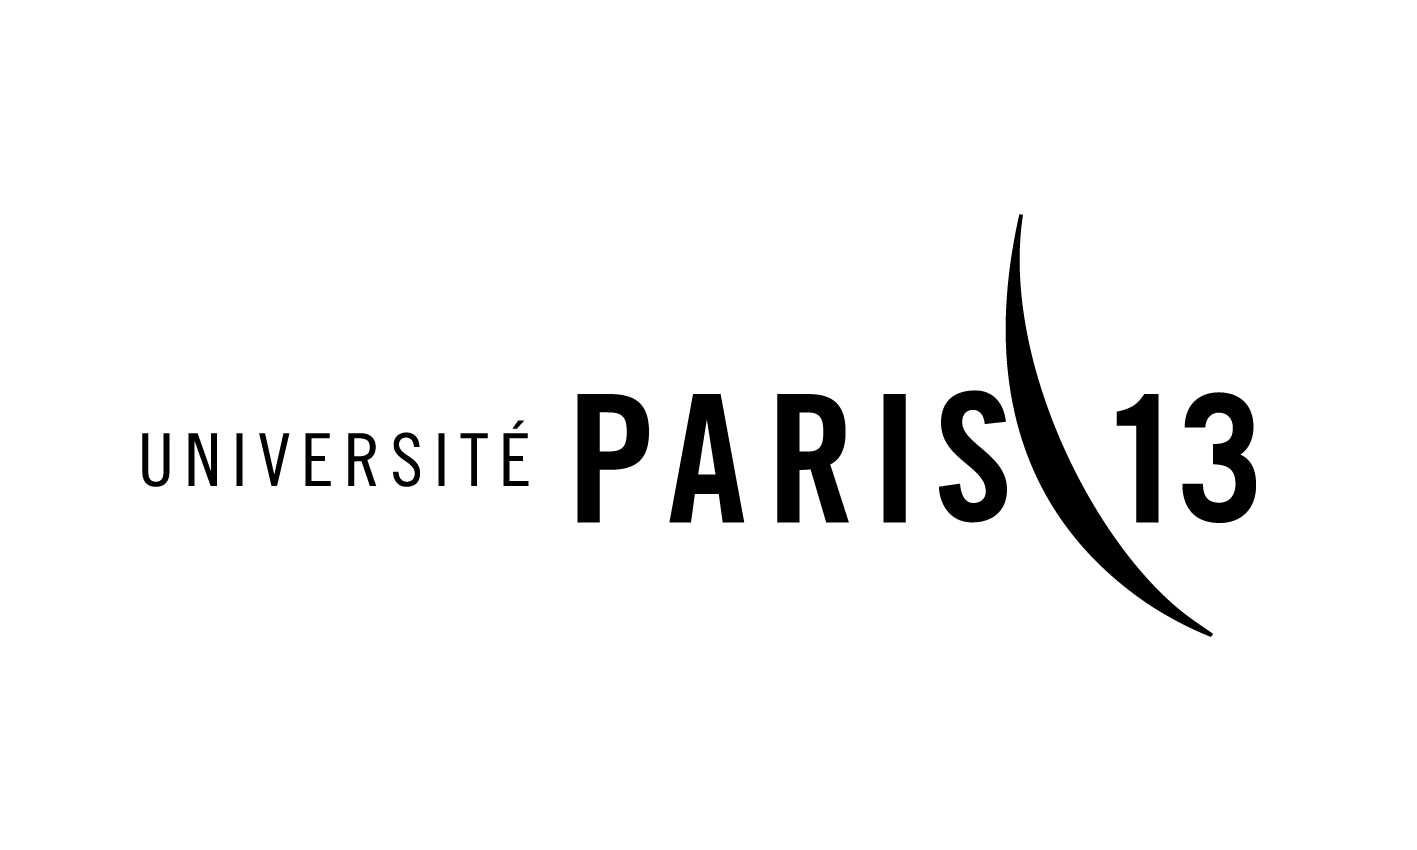
\includegraphics[width=30mm,scale=1]{UParis_13.png} \quad
 \vspace*{0.2in}
\titlepage
\end{frame}

\begin{frame}[label=guide]\frametitle{ Introduction }
Integration of renewable resources into the urban power grid is a challenge due to uncertainties in power production. We focus on wind power. Reliable wind power production forecasting is crucial to:
\begin{itemize}
\item \textbf{Optimization of the price of electricity} for different users such as electric utilities, Transmission system operator (TSOs), Electricity Service providers (ESPs), Independent power producers (IPPs), and energy traders.
\item \textbf{Allocation of energy reserves} such as water levels in dams or oil and gas reserves.
\item \textbf{Operation scheduling} of conventional power plants.
\item \textbf{Maintenance planning} such as that of power plants components and transmission lines.
\end{itemize}

\end{frame}

\begin{frame}\frametitle{Current State of Affairs}
  Wind power forecasts can be generally categorized as follows:
  \begin{itemize}
    \item physical models
    \item statistical methods
    \item artificial intelligence methods
    \item other hybrid approaches
  \end{itemize}
 The output of such methods is usually a \textcolor{red}{deterministic forecast}. \\
 \bigskip 
 Occasionally probabilistic forecasts are produced through uncertainty propagation or through forecast ensembles. \\
  \bigskip 
 However, there is a lacking in  \textcolor{red}{data driven stochastic forecasts} based on the real-world performance of forecasting models.
\end{frame}

\begin{frame}\frametitle{Data}
This is a year long data set from Uruguay based on \textbf{1000 72-hour long paths with observations recorded  every 10 min \textcolor{red}{ ($\sim$ half a million data points)}} recorded in 2018.
\begin{figure}
  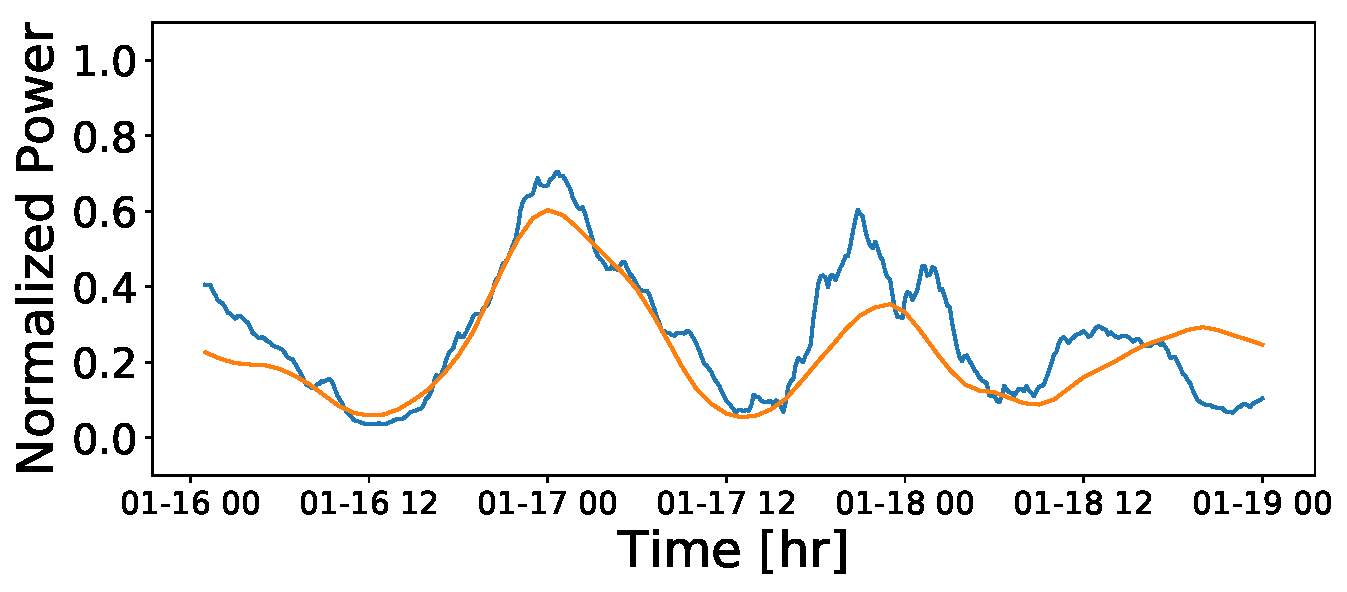
\includegraphics[width=70mm,scale=1]{plots/data_1516064400.pdf}
  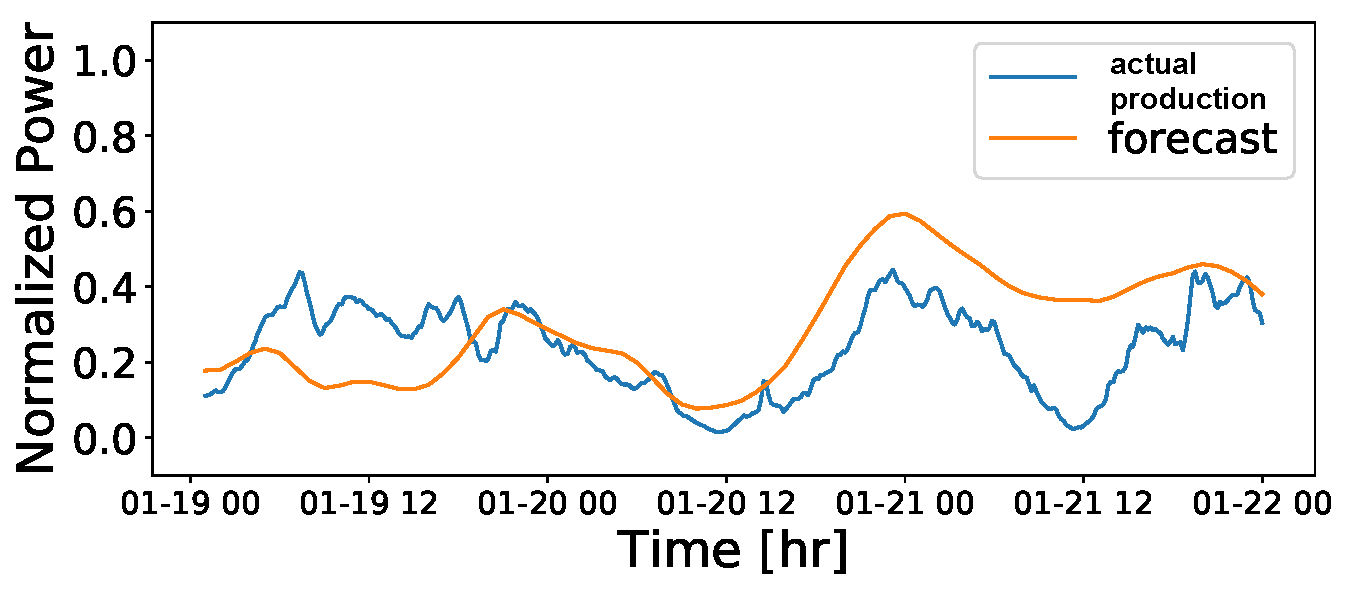
\includegraphics[width=70mm,scale=1]{plots/data_1516323600.pdf}\\
  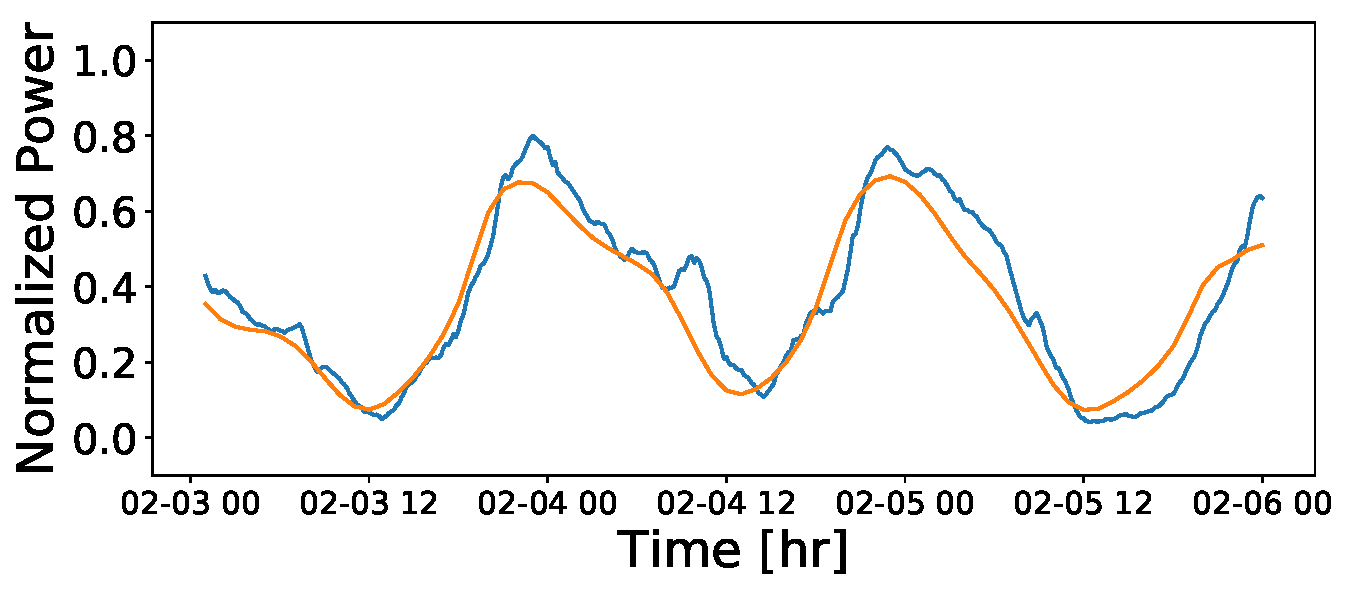
\includegraphics[width=70mm,scale=1]{plots/data_1517619600.pdf}
  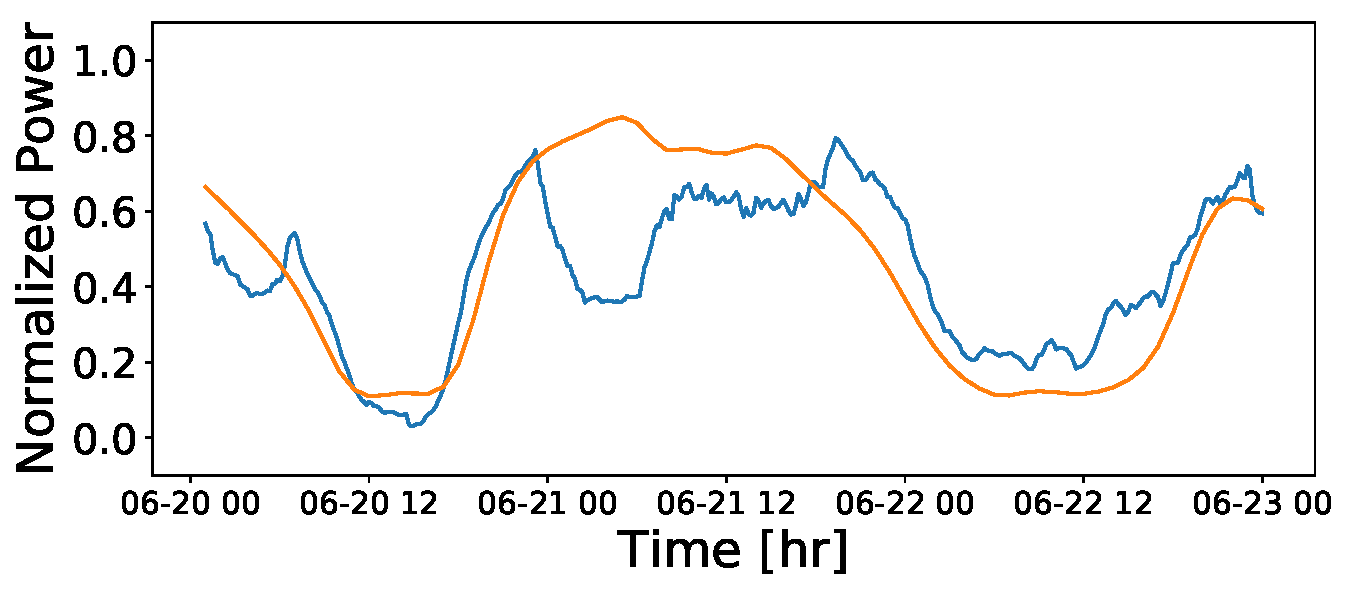
\includegraphics[width=70mm,scale=1]{plots/data_1529456400.pdf}
  % \caption{title}
\end{figure}
% Do you have more data? send it our way.
\end{frame}


\begin{frame}\frametitle{Data Skewness}
\begin{figure}
  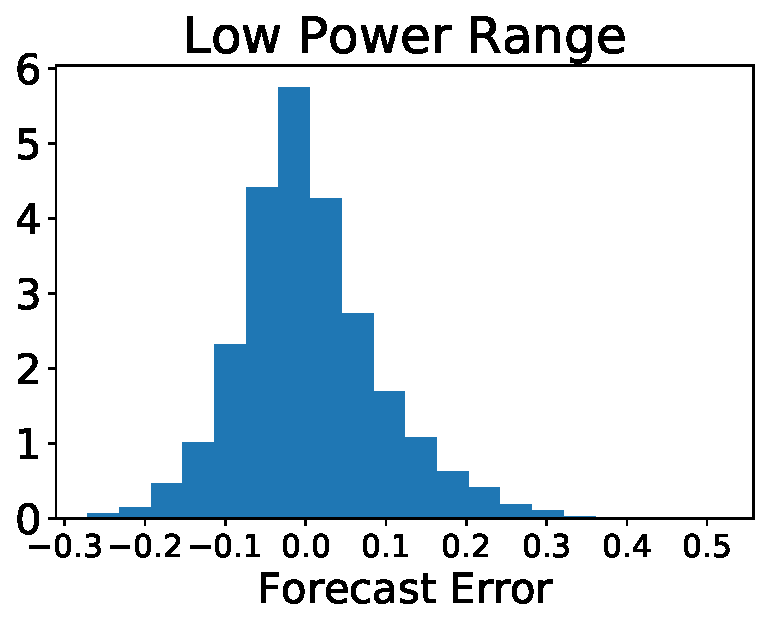
\includegraphics[width=47.5mm,scale=1]{plots/hist_low.pdf}
  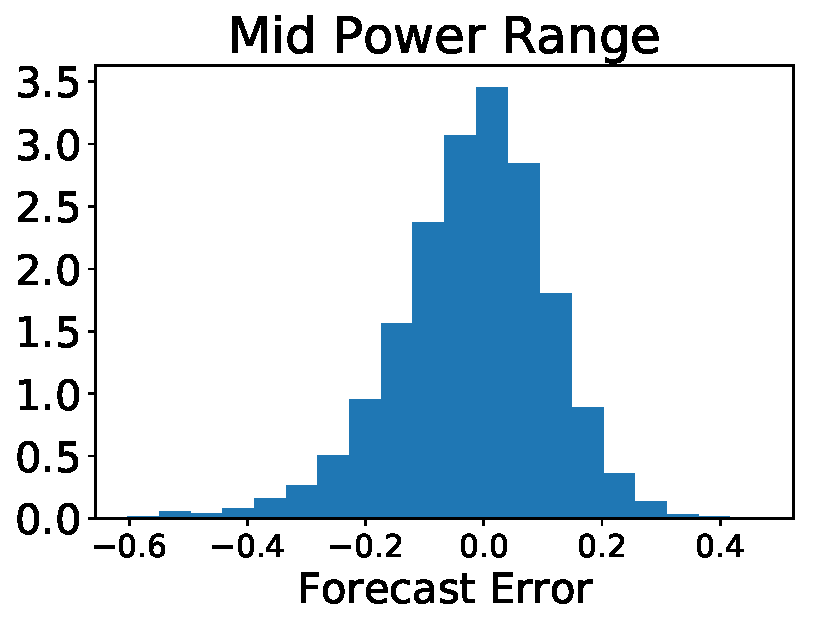
\includegraphics[width=50mm,scale=1]{plots/hist_mid.pdf}
  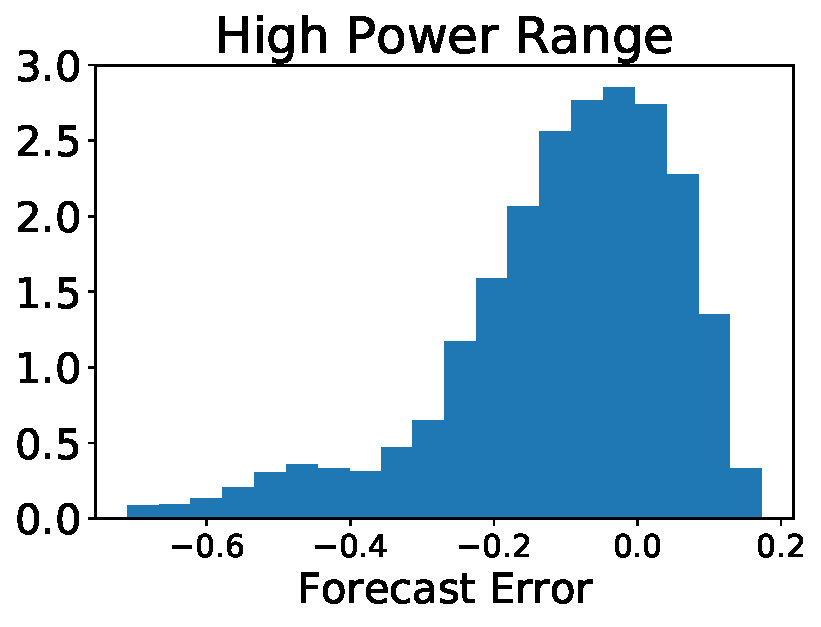
\includegraphics[width=50mm,scale=1]{plots/hist_high.pdf}
  \caption{We see that forecast errors exhibit \textcolor{red}{skewness} near the boundries (i.e. low and high power production regimes.)}
\end{figure}
\end{frame}

\begin{frame}\frametitle{Model}

Our goals are to produce a stochastic forecast of wind power production forecasting errors while:
\begin{itemize}
  \item Capturing the dynamics of the forecast error process.
  \item Capturing the skew nature of forecast errors.
  \item Being forecasting-technology agnostic. Thus, compatible with past and future forecasting-technology.
  \item Learning from historical power production data.
\end{itemize}
\end{frame}

\begin{frame}\frametitle{Model}
We propose to model wind power forecasts errors using \textcolor{red}{parametric stochastic differential equations (SDEs)} whose solution defines a stochastic process. This resultant stochastic process describes the time evolution dynamics of wind power forecasting errors.
\begin{equation}
\begin{split}
dX_t &= a(X_t; p_t, \dot{p}_t,\bm{\theta}) dt + b (X_t;p_t, \bm{\theta} ) dW_t \quad t > 0 \\
X_0 & = x_0
\end{split}
\label{main}
\end{equation}

\begin{itemize}
\item $a(\cdot; p_t, \dot{p}_t,\bm{\theta}):[0,1] \to \R $  a drift function.
\item $b (\cdot;p_t, \bm{\theta} ):[0,1] \to \R$  a  diffusion function.
\item $\bm{\theta}$: a vector of parameters.
\item $p_t$ time-dependent scalar value and $ \dot{p}_t$ is its time derivative at time $t$. (in our case  $p_t$ is a deterministic forecast).
\item $W_t$: Standard Wiener random process in $\R$.
\end{itemize}

\textcolor{blue}{Question: How do we choose an appropriate drift and diffusion functions?}

\end{frame}


\begin{frame}\frametitle{How do we choose an appropriate drift and diffusion functions?}

Let $\textcolor{red}{ \bm{\theta} }= (\textcolor{red}{\theta_0}, \textcolor{red}{\alpha})$
\begin{enumerate}
  \item We want the process to follow the wind forecast, thus we choose a drift term that is mean reverting and tracks the derivative of the deterministic forecast $p_t$, which is an input to our model.
  \begin{equation}
    a(x; p_t,\textcolor{red}{ \bm{\theta} })=  \dot{p_t} - \theta_t(x - p_t)
  \end{equation}
where $\theta_t>0$ is a time-dependent parameter that controls the speed of reversion.
  \item We want a diffusion term that vanishes at the boundaries to prevent the process from escaping the region $[0,1]$.
  \begin{equation}
    b (x; p_t,\textcolor{red}{ \bm{\theta} } )= \sqrt{2 \theta_t \textcolor{red}{\textcolor{red}{\alpha}} x (1-x)}
  \end{equation}
  where $\textcolor{red}{\alpha} >0$ is a constant parameter that controls the path variability.

To further ensure that the process does not escape the region $[0,1]$, the mean reversion parameter has to be selected according to the following rule,
\begin{equation}
\theta_t = \max \left( \textcolor{red}{\theta_0} \ , \ \frac{|\dot{p}_t|}{\min (p_t, 1-p_t)}  \right ),  \quad \textcolor{red}{\theta_0} >0 \label{theta_t}
\end{equation}
\end{enumerate}
\end{frame}

\begin{frame}\frametitle{Model}
Thus, our SDE becomes
\begin{equation}
\begin{split}
dX_t&= \dot{p}_t \ dt - \theta_t(X_t - p_t) \ dt + \sqrt{2 \theta_t \textcolor{red}{\alpha} X_t (1-X_t)}  \ dW_t \quad t > 0 \\
X_0&=x_0\\
% \theta_t &= \max \left( \textcolor{red}{\theta_0} \ , \ \frac{|\dot{p}_t|}{\min (p_t, 1-p_t)}  \right )\\
\end{split}
\label{model:derivative_tracking_X}
\end{equation}
To avoid differentiation of the forecast $p_t$ and simplify, we apply a change of variables $$V_t = X_t - p_t$$ \\
The  model becomes,
\begin{equation}
\begin{split}
dV_t &=  - \theta_t V_t \  dt + \sqrt{2 \theta_t \textcolor{red}{\alpha} (V_t +p_t ) (1-V_t-p_t)} \  dW_t  \\ %\quad t > 0
V_0 & = v_0\\
% \theta_t &= \max \left( \textcolor{red}{\theta_0} \ , \ \frac{|\dot{p}_t|}{\min (p_t, 1-p_t)}  \right )\\
\end{split}\label{VtSDE}
\end{equation}
Note that this model is \textcolor{red}{Markovian.}
\end{frame}

\begin{frame}\frametitle{Model}
Since $V_t$ defined by our SDE is Markovian, the \textcolor{red}{ likelihood function can be written as a product of transition densities}.  Consider a set of M paths with N observations each, $ V^{M,N}=\{ V_{t_1^{M,N}} , V_{t_2^{M,N}} ,\ldots , V_{t_N^{M,N}} \}$ observed in intervals of $\Delta_N$.

\begin{equation}
\mathcal{L}(\bm{\theta};V) =\prod\limits_{j=1}^M \prod\limits_{i=1}^N \rho ( {V_{j,i+1}|V_{j,i}},\textcolor{red}{ \bm{\theta} })  \rho (V_{j,0})
\label{likelihood}
\end{equation}

The transition densities can be exactly obtained by solving the following parametric Fokker-Planck equation,

\begin{equation}
\begin{split}
\frac{ \partial f }{\partial t } & (y ,t | x , s, \textcolor{red}{\theta_0} , \textcolor{red}{\alpha} )= - \frac{\partial}{ \partial y} ( a( y;  p_t, \dot{p}_t, \textcolor{red}{\theta_0} ) f( y ,t | x , s, \textcolor{red}{\theta_0}  , \textcolor{red}{\alpha} ) ) \\
& + \frac{1}{2} \frac{\partial^2}{ \partial y^2} ( b^2(y; p_t, \textcolor{red}{\theta_0}, \textcolor{red}{\alpha}  )  f(y ,t | x , s,\textcolor{red}{\theta_0} , \textcolor{red}{\alpha} ) ) \quad  t < s\\
\end{split}
\end{equation}
This is a parametric PDE which is \textcolor{red}{computationally expensive to solve} and optimize for every transition.
\end{frame}


\begin{frame}\frametitle{Moment Matching}
We propose a \textcolor{red}{proxy transition density}. We match the moments of our SDE model with that of the proxy density. Using It$\hat{o}$ formula, we arrive at the following iterative ODEs.

\begin{equation}
\begin{split}
\frac{d \E[ V^k_t]}{dt} = - k \theta_t \E [ V^k_t] + \frac{k(k-1)}{2} \E [ V^{k-2}_t  b(V^k_t;\theta_t, \textcolor{red}{\alpha})]
\end{split}
\end{equation}
For $t\in [t_{n-1}, t]$, the first two moments are given by
\begin{equation}
\begin{split}
\frac{d m_1 (t)}{dt} &= - m_1(t)\theta_t \\
\frac{d m_2 (t)}{dt} &=  -2 m_2(t)\theta_t(1+\textcolor{red}{\alpha}) + 2\textcolor{red}{\alpha}\theta_t m_1(t)(1-2p_t) + 2 \textcolor{red}{\alpha}\theta_t p_t (1-p_t)\\
\end{split}
\end{equation}
with initial conditions, $m_1(t_{n-1})= v_{n-1}$ and $m_2(t_{n-1})= v_{n-1}^2$.

 A suitable candidate is a \textcolor{red}{Beta transition } density as it is compactly supported and can morph into symmetric and asymmetric shapes.

\end{frame}

\begin{frame}\frametitle{Algorithm}

Execute the following until an accuracy threshold is met:
\begin{enumerate}
\item \textcolor{red}{initialize}.
\item \textcolor{red}{optimize} the log-likelihood function.
\begin{enumerate}
\item For every evaluation of the log-liklihood function:
\begin{enumerate}
  \item \textcolor{red}{Sample} a mini-batch of transitions randomly with their associated forecast and parameters.
  \item \textcolor{red}{Solve} the ODE system for every transition to obtain the moments.
  \item \textcolor{red}{Match} the resulting moments with the parameters of the chosen proxy distribution for every transition.
\end{enumerate}
\end{enumerate}
\item go to step 1 (i.e. \textcolor{red}{re-initialize} the optimization with the most recent result ).
\end{enumerate}

In the above:
\begin{itemize}
\item Choose your favorite deterministic optimization algorithm.
\item Choose your favorite integrator to solve the ODE system.
\end{itemize}
\end{frame}

\begin{frame}\frametitle{Inference Results}
% Here we show the convergence path of the optimization in 2D, the likelihood in 3D and rate of the shrinking ellipses in one slide.

\begin{figure}
  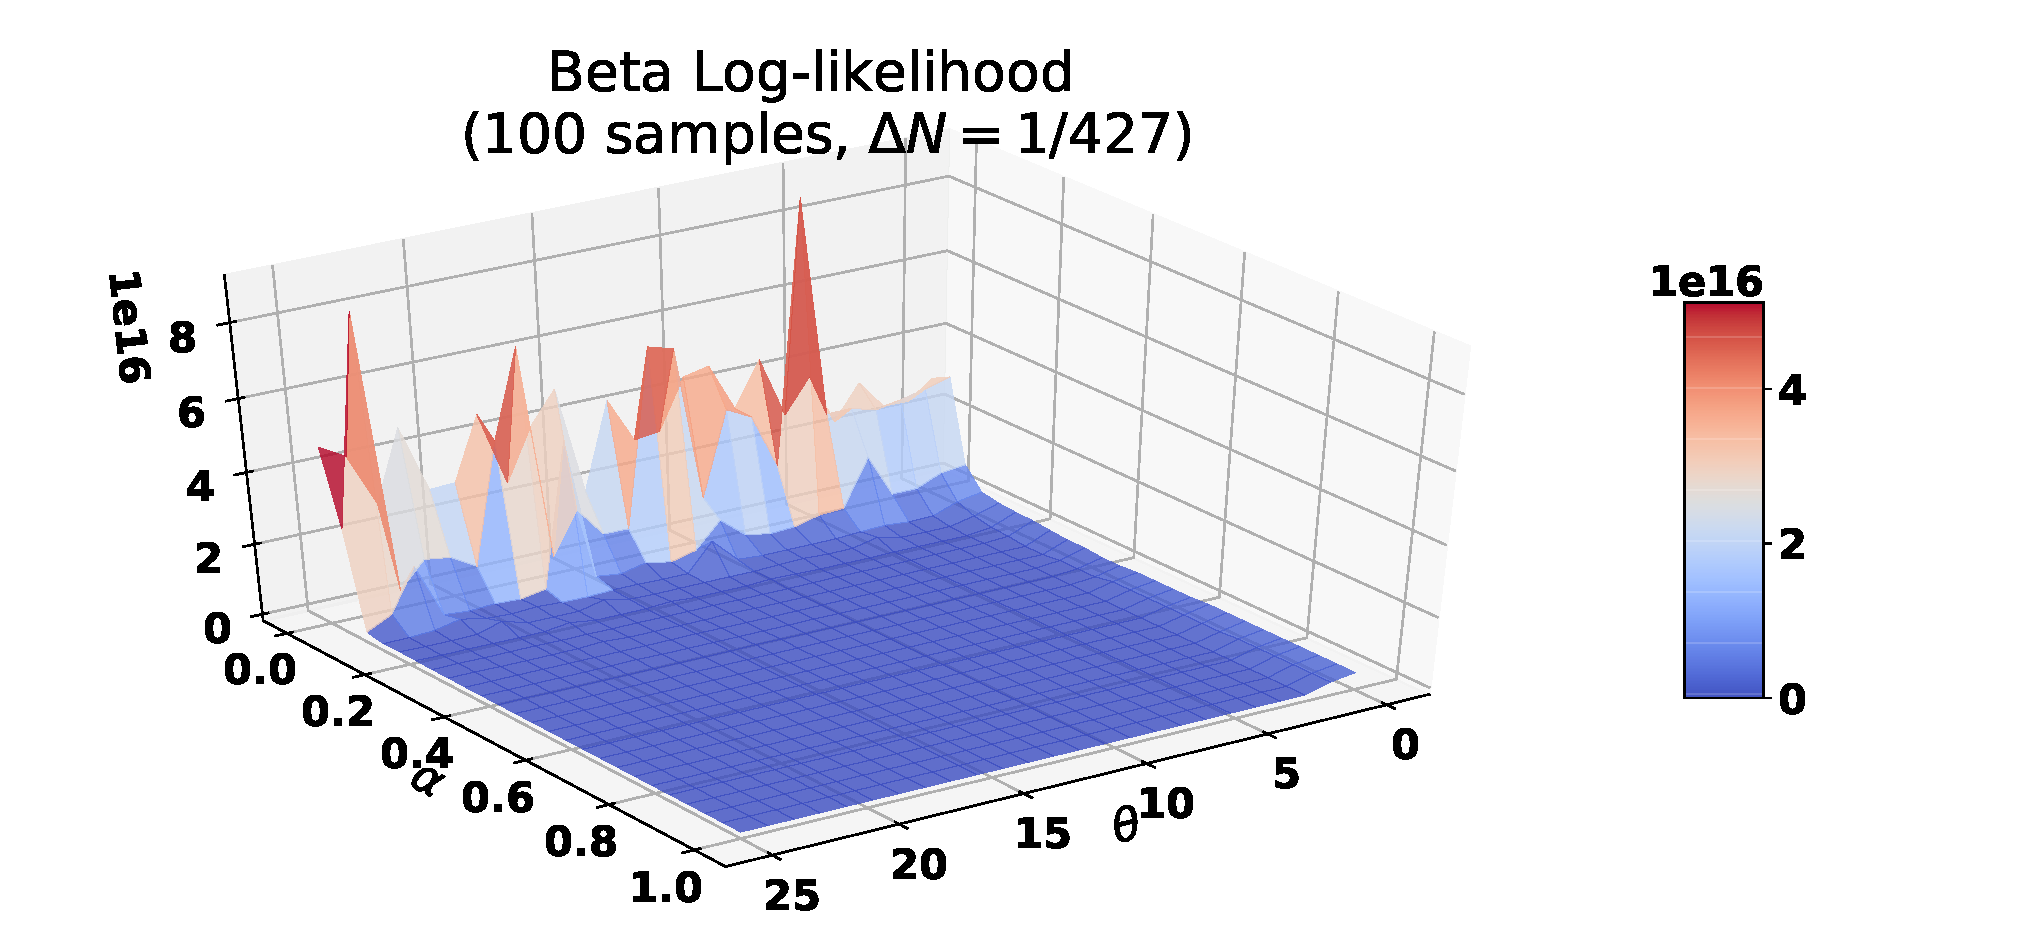
\includegraphics[width=110mm,scale=1]{plots/beta_likeli_3d.pdf}
  \caption{3-D view of the \textcolor{red}{inverted beta log-likelihood}  function of 100 sample paths. That is a total of  \textcolor{red}{ $\sim 42,700$ data points }}
\end{figure}
\end{frame}


\begin{frame}\frametitle{Inference Results}
\begin{figure}
  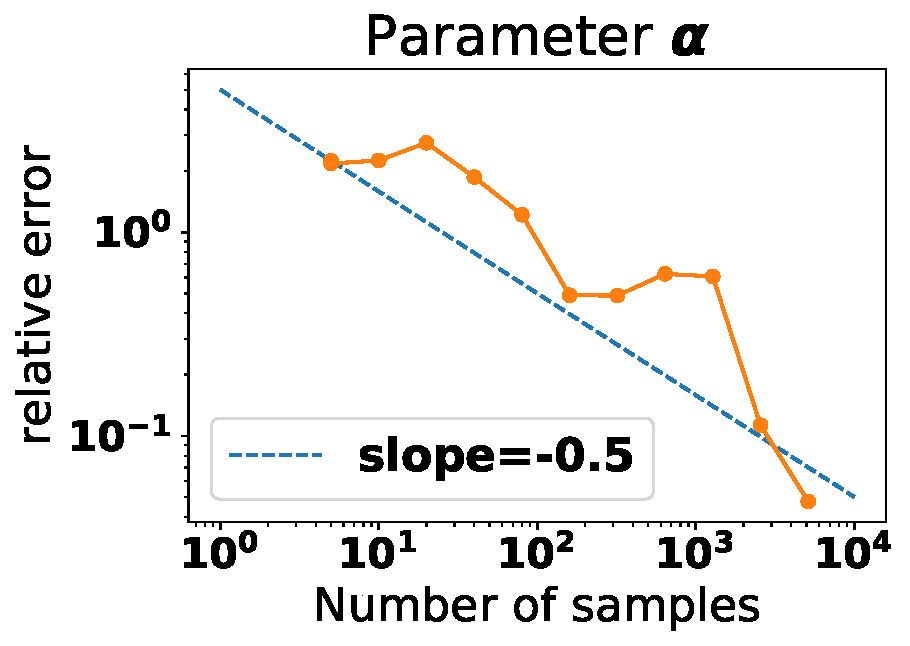
\includegraphics[width=70mm,scale=1]{plots/alpha_conv_beta.pdf}
  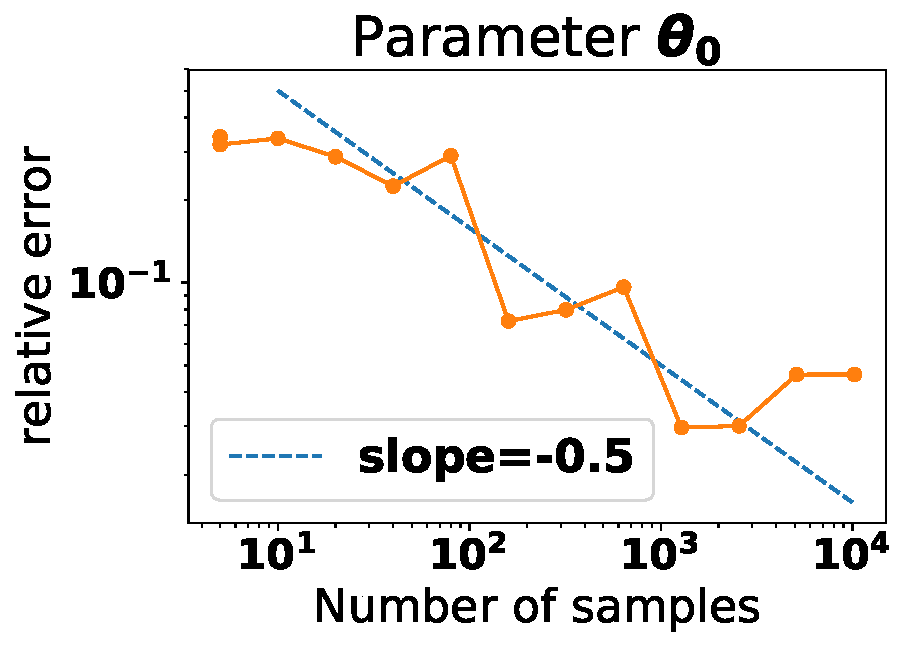
\includegraphics[width=70mm,scale=1]{plots/theta_conv_beta.pdf}
  \caption{We have \textcolor{red}{self-convergence} of our algorithm at a rate that matches the convergence rate of Monte Carlo.}
\end{figure}
\end{frame}

\begin{frame}\frametitle{Future Wind Power Simulation}
    \begin{figure}
      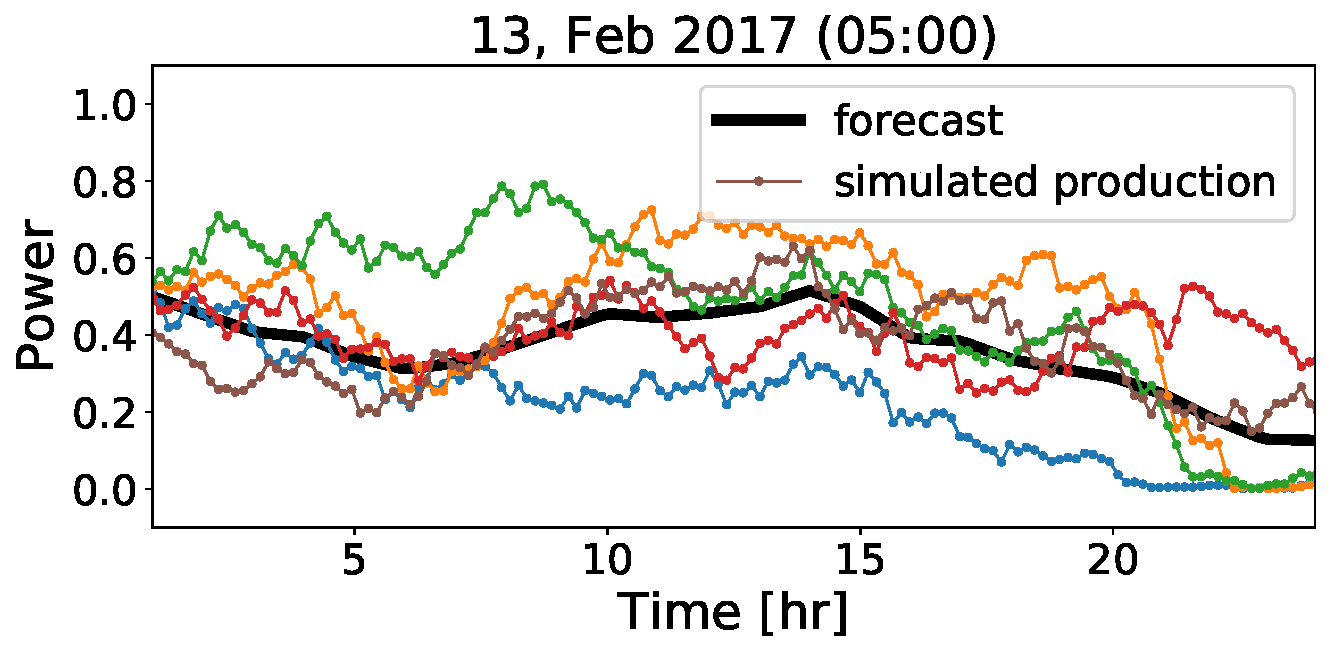
\includegraphics[width=75mm,scale=1]{simulated/24hr/1099.pdf}
      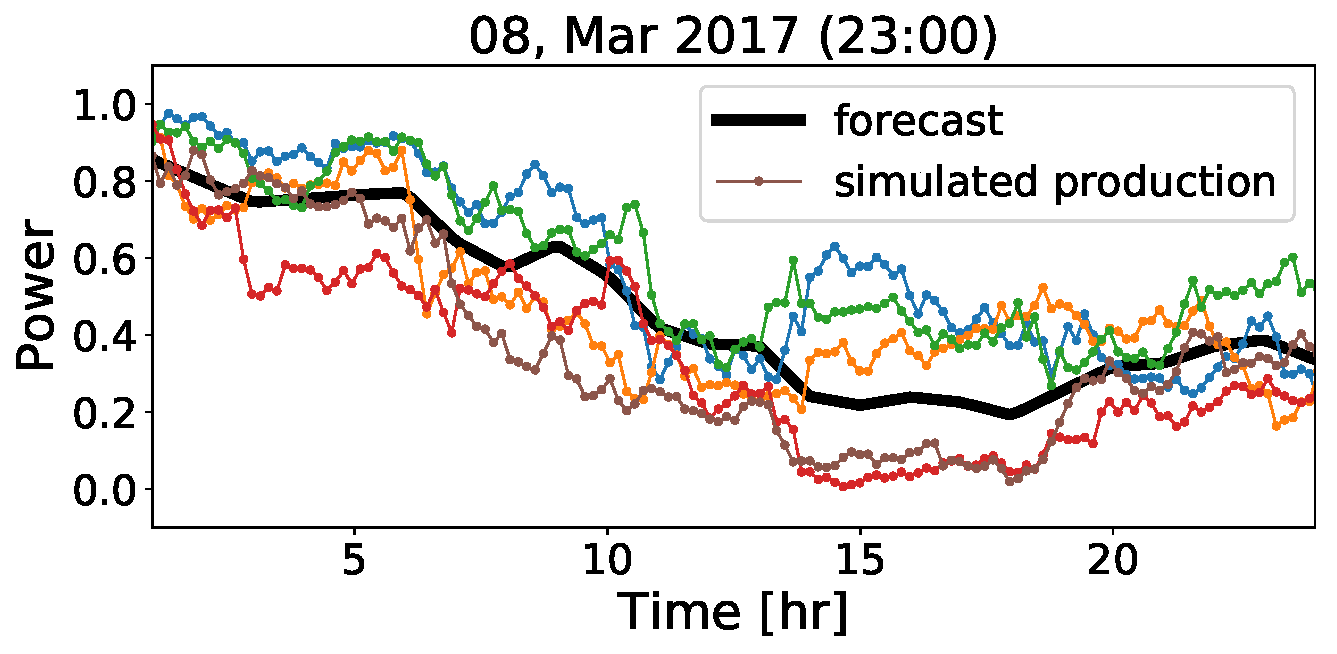
\includegraphics[width=75mm,scale=1]{simulated/24hr/1178.pdf}
      \caption{We simulate five possible future wind power production paths using the obtained optimal parameters $(\textcolor{red}{\theta_0}, \textcolor{red}{\alpha} )=(12,0.3)$ }
    \end{figure}
\end{frame}


\begin{frame}\frametitle{Confidence Bands}
    \begin{figure}
      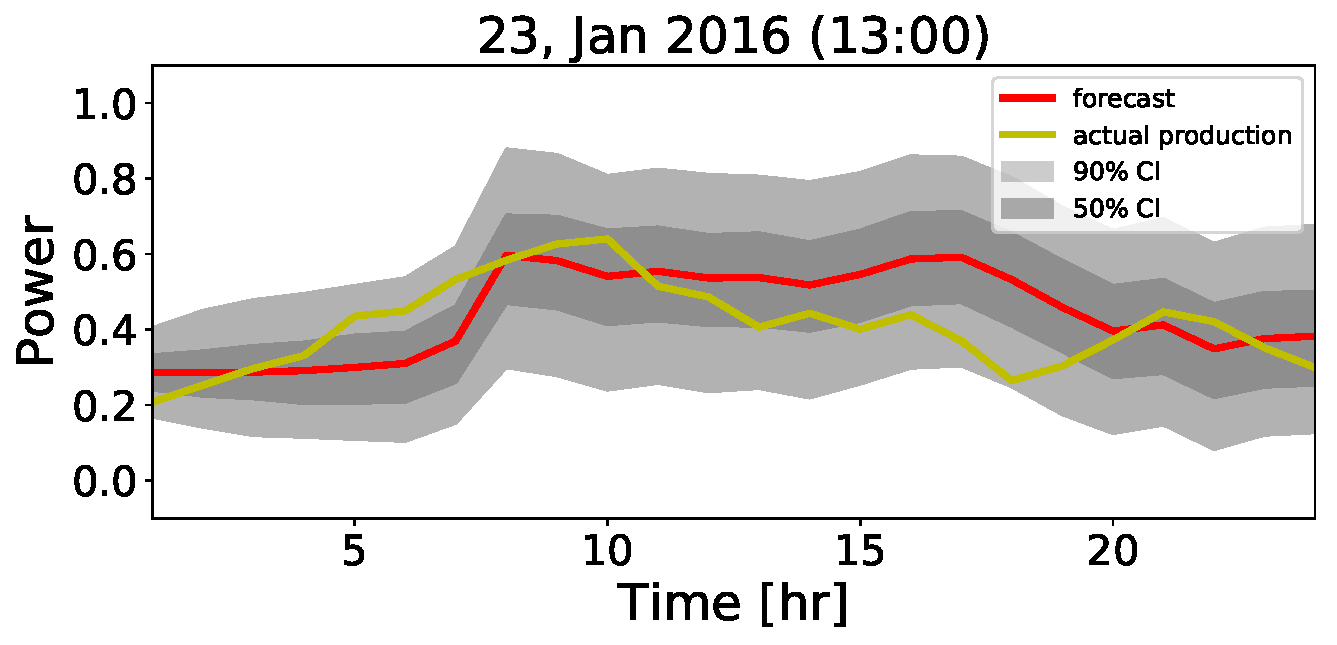
\includegraphics[width=75mm,scale=1]{confidence_intervals/24hr/31.pdf}
      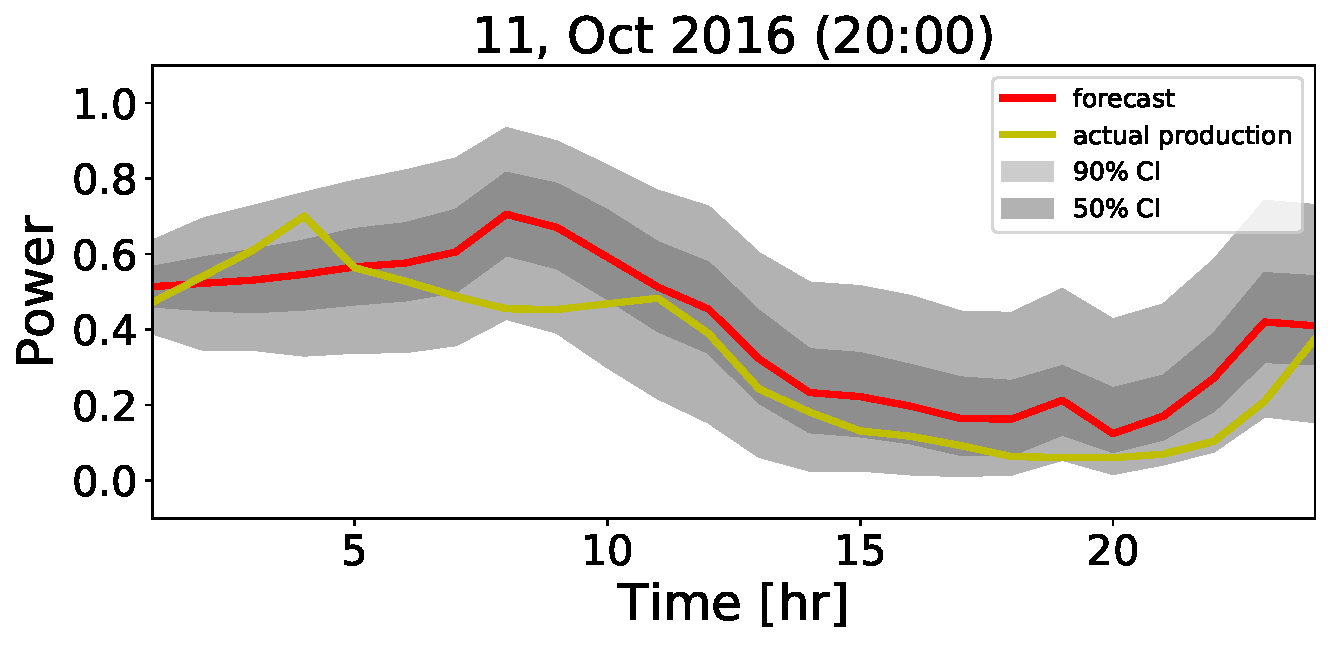
\includegraphics[width=75mm,scale=1]{confidence_intervals/24hr/820.pdf}
       \caption{We obtain confidence intervals for future wind power production using the obtained optimal parameters $(\textcolor{red}{\theta_0}, \textcolor{red}{\alpha} )=(12,0.3)$. Actual production plotted in retrospect. }
    \end{figure}
\end{frame}

\begin{frame}\frametitle{State-Independent Diffusion Formulation}
The model we have demonstrated previously is \textcolor{red}{state-dependent diffusion} formulation, that is the diffusion of the SDE depends on the state.
\begin{equation}
\begin{split}
dV_t &=  - \theta_t V_t \  dt + \sqrt{2 \theta_t \textcolor{red}{\alpha} (V_t +p_t ) (1-V_t-p_t)} \  dW_t  \\ %\quad t > 0
V_0 & = v_0\\
\end{split}\label{VtSDE}
\end{equation}

Why are we interested in a state-independent diffusion formulation? Because it's more tractable and numerically stable.\\
We apply a \textbf{Lamperti transform} to obtain the following \textcolor{red}{state-independent diffusion} SDE,

\begin{equation}
  \begin{split}
    dZ_t&= \frac{- \theta_t (1+ \sin(Z_t) - 2p_t) + \textcolor{red}{\alpha} \theta_t \sin (Z_t)   }{\cos (Z_t)} \ dt + \sqrt{2 \textcolor{red}{\alpha} \theta_t} dW_t \\
    Z_0&=z_0
  \end{split}
\end{equation}
where $Z_t = \arcsin \left( \frac{1}{2} \left( V_t+p_t \right) - 1 \right) $.
\end{frame}

\begin{frame}\frametitle{Data Skewness after Lamperti Transformation}
As stated before, the state-independent diffusion SDE follows a Lamperti transformed process $Z_t$ given by $Z_t = \arcsin \left( \frac{1}{2} \left( V_t+p_t \right) - 1 \right) $.
\begin{figure}
  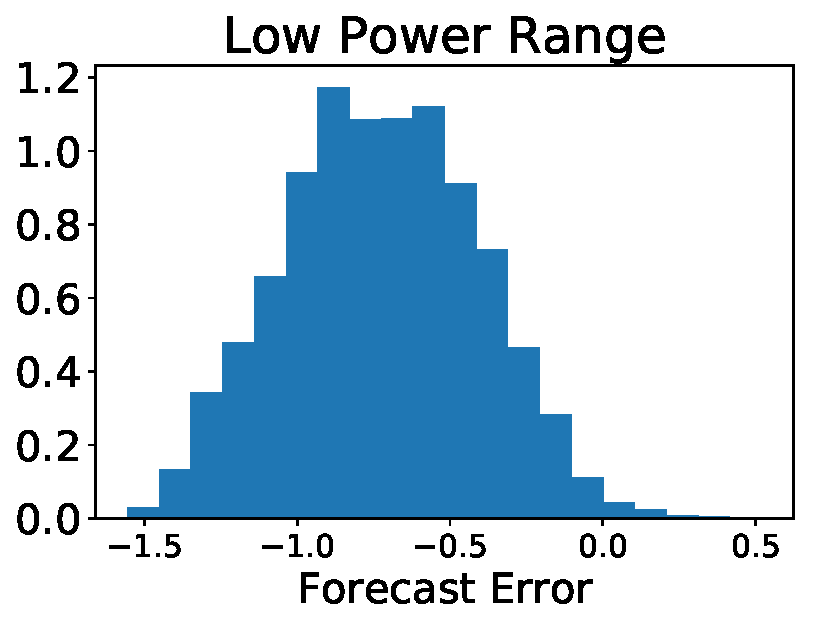
\includegraphics[width=50mm,scale=1]{plots/hist_low_lamperti.pdf}
  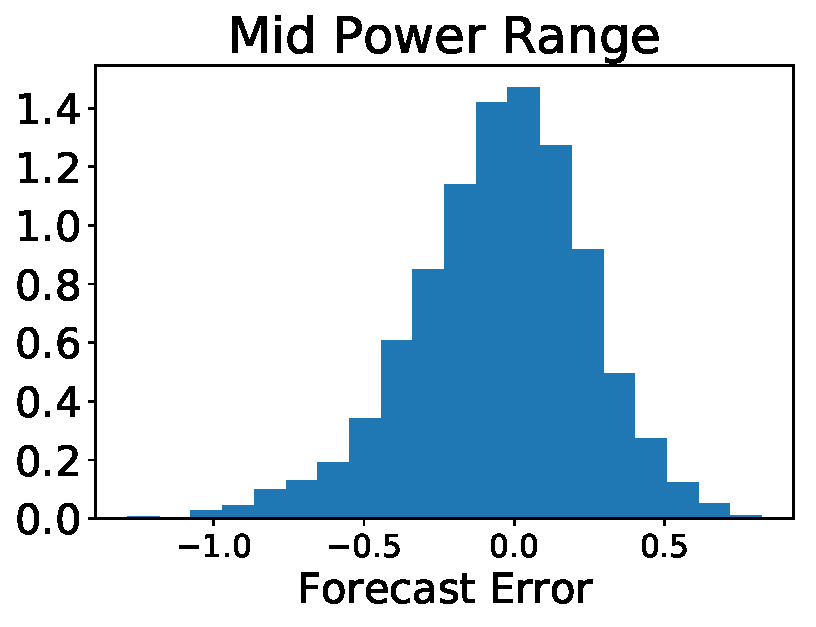
\includegraphics[width=50mm,scale=1]{plots/hist_mid_lamperti.pdf}
  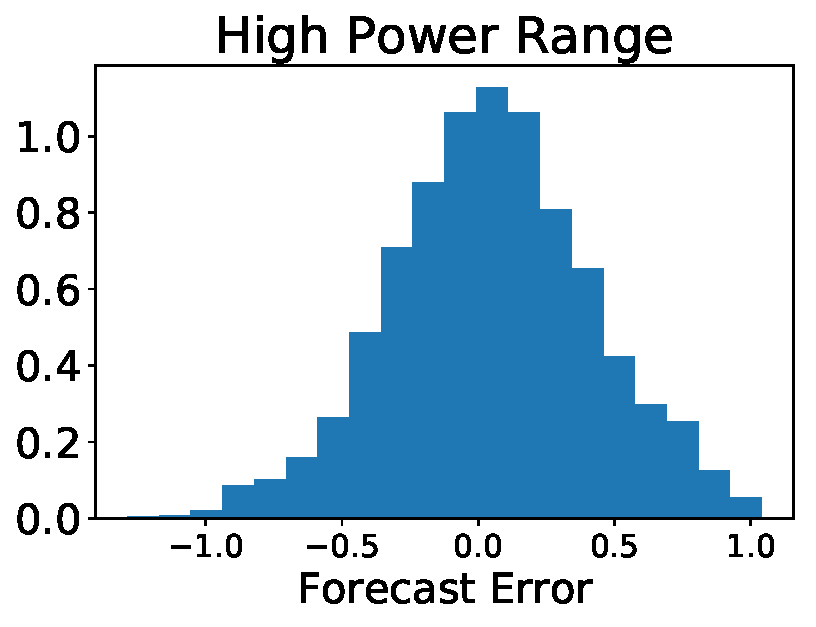
\includegraphics[width=50mm,scale=1]{plots/hist_high_lamperti.pdf}
  \caption{We observe that skewness has been greatly reduced after the Lamperti transformation. This motivates us to use a \textcolor{red}{Gaussian transition} density as a proxy density.}
\end{figure}
\end{frame}

\begin{frame}\frametitle{State-Independent diffusion formulation}
Similarly, we try to obtain a system of ODEs to determine the centered moments of the Lamperti transformed process $V_t$. Due to the non-linearity in the drift, we can only approximate the centered moments by the following ODEs,
\begin{equation}
\begin{split}
\frac{d m_1 (t)}{dt} &= - m_1(t)\theta_t (1-\textcolor{red}{\alpha}) - \theta (1-2 p_t) \\
\frac{d var(t)}{dt} &=  2 var(t) \theta_t (2p_t - 1 ) \tan(m_1 (t)) \sec(m_1 (t)) + \theta_t (\textcolor{red}{\alpha} - 1) \sec^2(m_1 (t))  + 2 \theta_t \textcolor{red}{\alpha}\\
\end{split}
\end{equation}
with initial conditions, $m_1(t_{n-1})= v_{n-1}$ and $var(t_{n-1})= v_{n-1}^2 - v_{n-1}$.\\
\bigskip 
\textcolor{red}{These are not exact ODEs for the centered moments}, however they are accurate enough for small time intervals. 
\end{frame}



\begin{frame}\frametitle{Result Comparison in the Different Spaces}
\begin{table}[]
\centering
\begin{tabular}{|c|c|}
\hline
Formulation   &  parameters $(\textcolor{red}{\theta_0}, \textcolor{red}{\alpha})$    \\ \hline
Without Lamperti transform &   $(12,0.3) $   \\ \hline
With Lamperti transform &   $(12,0.29)  $   \\ \hline
\end{tabular}
\caption{We compare the parameters obtained in both the original and Lamperti space. }
\label{tab:model_comparison}
\end{table}
\end{frame}

\begin{frame}\frametitle{Concluding Remarks}
We were able to:
\begin{itemize}
  \item simulate future wind power production based on real data.
  \item obtain an analytical description of the uncertainty of wind power forecasts in the form of an SDE.
  \item develop a forecasting technology agnostic method.
  \item capture skewness of the error process and its dynamics.
\end{itemize}
\end{frame}


\begin{frame}\frametitle{References}


\section*{References}
\begin{flushleft}
\begin{itemize}
\item Alhaddad, W. ,  Kebaier, A. , \& Tempone, R. (2019). Stochastic Wind Power Forecasting. In preparation.
\item  M\o ller, J. K., Zugno, M., \& Madsen, H. (2016). Probabilistic Forecasts of Wind Power Generation by Stochastic Differential Equation Models. Journal of Forecasting, 35(3), 189-205. doi:10.1002/for.2367 
\item  Elkantassi, S., Kalligiannaki, E., \& Tempone, R. (2017). Inference And Sensitivity In Stochastic Wind Power Forecast Models. Proceedings of the 2nd International Conference on Uncertainty Quantification in Computational Sciences and Engineering (UNCECOMP 2017). doi:10.7712/120217.5377.16899
\item Giebel, G., Brownsword, R., Kariniotakis, G., Denhard, M., \& Draxl, C. (2011). The State-Of-The-Art in Short- Term Prediction of Wind Power: A Literature Overview, 2nd edition. ANEMOS.plus. https://doi.org/10.11581/DTU:00000017 
\item Chang, W.-Y. (2014) A Literature Review of Wind Forecasting Methods. Journal of Power and Energy Engineering, 2, 161-168. http://dx.doi.org/10.4236/jpee.2014.24023
\end{itemize}
\end{flushleft} 

\end{frame}


\end{document}
